\chapter{開発プロセス}

\section{ヒアリング}
我々は町会の置かれている現状を明らかにするため、
5月12日に町会の会長、副会長、総務部長、会計部長、青少年育成部副部長に対して、
我々は学部3年生5名とTA5名と教員4名でヒアリングを行った。
町会役員から\ref{problems}で述べたイベント開催に関する問題と以下の要望が明らかになった。

\begin{itemize}
\item 開催予定のイベント一覧をカレンダーで表示して欲しい。
\item iOSのアプリケーションを作って欲しい。
\item 幅広い年代の人が使いやすいUIにして欲しい。
\item 町会の役員の数を増やすため、町内会を知ってもらいたい。
\item イベント発信をした際に通知できる機能が欲しい。
\item イベントスケジュールでイベントの削除、作成、更新ができるようにして欲しい。
\item 行事をタップしたらそのまま参加申し込みフォームに遷移して欲しい。
\item 保護者の方の確認を得るためのポップアップ機能が欲しい。
\item イベントで不参加になった人が分かるようにして欲しい。
\end{itemize}

我々は、これらの要望を取り入れつつ問題を解決するアプリケーションを開発することとした。
\bunseki{永井陽太}


\section{アプリケーションアイデアの考案}
\ref{problems}で述べた問題と町会の要望を分析した結果、イベントに関する内容のものが多かった。
そこでイベントに関係する3つの問題を解決することとした。問題は
「FacebookやLINE@ではイベントに関するお知らせはできるが、開催予定のイベントを一覧で見れない」
「Facebookでは個人情報が漏れてしまうため参加申し込みができない」
「役員だけで共有したい情報を町民に知られずに共有することがFacebookやLINE@ではできない」の3つである。
これらの問題を解決するために、開催予定イベントのカレンダー表示機能、
イベントへの参加申し込み機能、参加申し込み者の情報を役員のみが見ることのできる機能、
役員のみが役員会議などのイベント情報を見ることのできる機能を考案した。
アプリケーションアイデアの一部であるイベントカレンダー画面(図\ref{calender})、
参加フォーム画面(図\ref{joinform})、イベント作成画面(図\ref{create_event.old})を以下に示す。

\newpage
\begin{figure}[h]
    \begin{tabular}{ccc}
      %---- 最初の図 ---------------------------
      \begin{minipage}[t]{0.33\hsize}
        \centering
        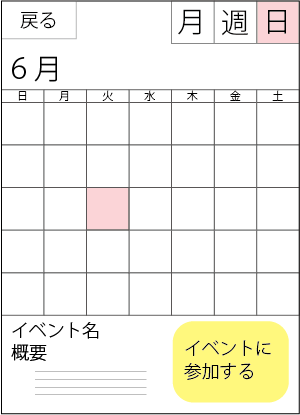
\includegraphics[keepaspectratio, scale=0.4]{process_figures/calender.png}
        \caption{イベントカレンダー画面}
        \label{calender}
      \end{minipage} &
      %---- 2番目の図 --------------------------
      \begin{minipage}[t]{0.33\hsize}
        \centering
        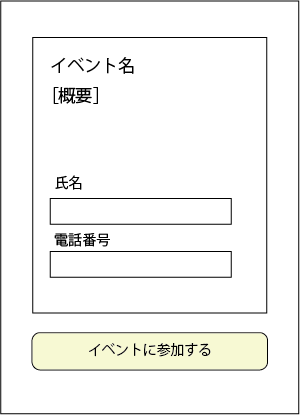
\includegraphics[keepaspectratio, scale=0.4]{process_figures/joinform.png}
        \caption{参加フォーム画面}
        \label{joinform}
      \end{minipage}
      %---- 3番目の図 --------------------------
      \begin{minipage}[t]{0.33\hsize}
        \centering
        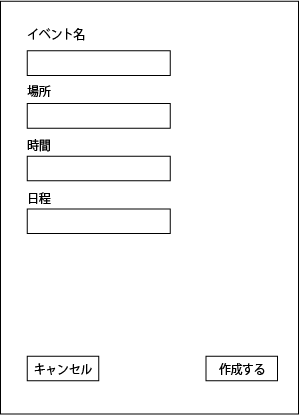
\includegraphics[keepaspectratio, scale=0.4]{process_figures/old_create_event.png}
        \caption{イベント作成画面}
        \label{create_event.old}
      \end{minipage}
      %---- 図はここまで ----------------------
    \end{tabular}
\end{figure}
\bunseki{永井陽太}

\section{第1回提案}
\label{first_review}
5月30日に我々が考えたアプリケーションの画面イメージを町会に提案した。
その結果、iOS、Android、Webアプリケーションの3つに対応可能なアプリケーション開発を行うことが決定した。
また、我々の考案したアプリケーションイメージについて、レビューで3つの要望を得た。
1つ目は、イベント参加者の名簿を市役所に提出する際に参加者の情報として「名前」「性別」「年齢」「住所」「電話番号」が必要なので、
図\ref{joinform}の入力フォームに5つの情報を追加して欲しいという要望である。
2つ目は、アプリケーションをインストールした人が、すぐイベントを確認できるように起動時の画面はログイン画面にしないで欲しいという要望である。
3つ目は、図\ref{create_event.old}に「定員」の項目を追加して欲しいという要望である。
\bunseki{永井陽太}

\section{アプリケーションアイデアの改善}
\ref{first_review}のレビューの内容を参考にしてアプリケーションアイデアを改善した。
この改善に対して、6月に行われたプロジェクトグループ内月例レビューにて、
役員と町民でイベントカレンダーを共有することで本当に問題を解決できるのかと教員より指摘を受け、
アプリケーションについて再考し改善を図った。その結果、カレンダーを用いて開催予定のイベントを表示するのではなく、
開催予定のイベントを直近のものから順にリスト表示することにした。
なぜなら、カレンダー表示では来月の予定などがひと目で確認することができないからである。
アプリケーションアイデアの一部であるイベントリスト画面(図\ref{eventlist})、
イベント作成画面(図\ref{new_create_event})、参加者リスト画面(図\ref{joinedlist})を以下に示す。

\newpage%苦肉の策
\begin{figure}[h]
    \begin{tabular}{ccc}
      %---- 最初の図 ---------------------------
      \begin{minipage}[t]{0.3\hsize}
        \centering
        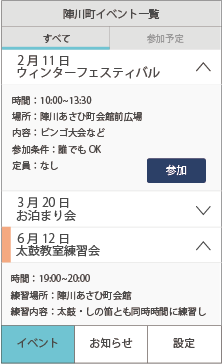
\includegraphics[keepaspectratio, scale=0.5]{process_figures/eventlist.png}
        \caption{イベントリスト画面}
        \label{eventlist}
      \end{minipage} &
      %---- 2番目の図 --------------------------
      \begin{minipage}[t]{0.3\hsize}
        \centering
        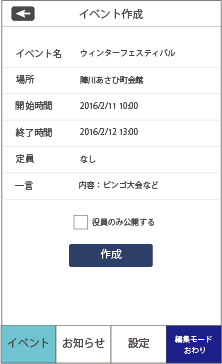
\includegraphics[keepaspectratio, scale=0.5]{process_figures/new_create_event.png}
        \caption{イベント作成画面}
        \label{new_create_event}
      \end{minipage}
      %---- 3番目の図 --------------------------
      \begin{minipage}[t]{0.3\hsize}
        \centering
        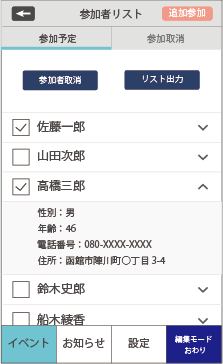
\includegraphics[keepaspectratio, scale=0.5]{process_figures/joinlist.png}
        \caption{参加者リスト画面}
        \label{joinedlist}
      \end{minipage}
      %---- 図はここまで ----------------------
    \end{tabular}
\end{figure}
\bunseki{永井陽太}

\section{第2回提案}
6月23日に我々は町会に対して改善したアプリケーションイメージを提案した。
その結果、画面ごとにレビューしてもらい詳細な要望を受けた。
具体的には、図\ref{eventlist}でイベントをタップすると画面いっぱいにイベントの詳細情報が表示されるようにして欲しいという要望、
図\ref{new_create_event}にアプリケーションの所有者全員に通知するか、しないかの項目を設けて欲しいという要望である。
また、町民が利用したくなるようなコンテンツを追加して欲しいという要望も得た。
過去のイベントの写真が確認できるWebページとアプリケーションとリンクさせることが例として挙げられる。
\bunseki{永井陽太}
